
\subsection{Command line interface} % (fold)
\label{sub:command_line_interface}

Firstly, a note has to be made on the general choice of implementation
of the command line interface.
Following \textsc{Unix} command line style, one should be able to run
a command with multiple arguments in the following
style \lstinline|command -arg1_type arg1 -arg2_type arg2|.
In the \MyFoodora~case, it seems more adequate to have one syntax for each
command, being \lstinline|command <arg1> <arg2>|, which is proposed in 
the project requirements. The program will thus be able to give informations
on the commands when needed and we expect the user to quickly remember 
the commands, as there is only few of them for each user type.
 
The choice of implementation described in the first paragraph
lead us to the use of an \lstinline|HashMap<String, Integer>| to
store the list of commands and their associated number of arguments,
as we only have \emph{one} number of arguments for one command,
except for the \lstinline|showTotalProfit| method which is handled
simply by using \lstinline|null| when no dates are given.

In terms of effeciency, using a parallel \lstinline|HashMap| to store
the commands names and their associated number of needed arguments,
allows to check if the given command name exists in $\mathcal{O}(1)$
time on average and in $\mathcal{O}(\log{n})$ on worst case~\cite{hashMap}.

\subsubsection{Separing interpretor from processor} % (fold)
\label{sub:separing_command_getter_and_command_processor}

Thinking about the design, we quickly found a need to separate
the \emph{request} (ie. the given command) from its actual \emph{execution}.
This idea follows the open/close principle and has similar advantages
as design patterns (note that we discovered the \emph{command design pattern}~\cite{wiki:commandPattern} which is somewhat similar).
It indeed allows to easily change the behaviour of the program if
one wants to change the syntax of the commands (\emph{request} class)
or what a particular command does (\emph{execution} class).
This lead to the implementation of the \CommandLine~and
the \CommandProcessor~classes.

In order to make use of commands in an efficient way,
a \Command~class is designed.
It consists of a name and an array
of strings containing its arguments.
This allows the interpretor and processor to easily
communicate between themselves and with the real user.
The reader is advised to have a look at figure~\ref{fig:clui_uml}
containing the UML diagram of the relationship between
the three listed above classes.
One will notice the use of the Singleton pattern for
the \CommandProcessor~and \CommandLine.
This is justified by the fact that only one
of each will be required at the same time
and it does not created problems with \textsc{JUnit} tests
as those are made using concrete scenarios
generated by \texttt{.txt} files of commands.
% subsubsection separing_command_getter_and_command_processor (end)

\subsubsection{The \texttt{CommandLine} class} % (fold)
\label{ssub:the_commandline_class}
The \CommandLine~can be seen as the \emph{interpreter}. It will be the link
class between the real user and the system. It can either interpret commands
given directly as input with the \lstinline|launchFromInput()| method,
or listed in a \texttt{.txt} file with the \lstinline|launchFromFile| method.
Once a String that should represent a command is given to those methods,
they will call the \lstinline|getInputInfoAndProcessCmd| method whose
role is to check if the input
\begin{enumerate}
  \item corresponds to an existing command,
  \item has the ``$<>$'' argument declaration,
  \item has the right number of arguments associated with this command. 
\end{enumerate}
If one of those conditions is not satisfied, a message containing the
error description will be send back to the \lstinline|launch| method
which will print it.
On the other hand, if the conditions are satisfied, the method
creates a new \Command~object and pass it to the \lstinline|processCmd|
method of its \CommandProcessor~attribute.
% subsubsection the_commandline_class (end)

\subsubsection{The \texttt{CommandProcessor} class} % (fold)
\label{ssub:the_commandprocessor_class}
The \CommandProcessor~can be seen as the \emph{executor}.
When its \lstinline|processCmd| receives a \Command~(which
is valid thanks to the \CommandLine),
it executes the behavior associated with the given command.
It's attributes mainly consist of the \Core~system,
as most of the method will need it and of 
a \lstinline|DishFactory| and a \lstinline|MealFactory|
that will be used to produces meals and dishes efficiently.

The methods of this class will mostly consists of translation
of user commands into \Core~commands.
One will note that not all user commands are available in
the core but are directly applicable to the \lstinline|current_user|
of the core. For example when a courier wants to set his status
to \emph{avaible},
one simply executes \lstinline|core.getCurrent_courier().setAvailable(true)|.

Now will be described how the \emph{creation of meals and orders} is handled. 
As we are required to create meals and orders
using multiple commands in the following pattern
\begin{enumerate}
  \item create a new \Meal~or \Order~giving basic information
  \item add dishes (resp. items) to \Meal~(resp. \Order)
  \item validate steps 2 and 3 by using a \lstinline|save| like function
\end{enumerate}
we used \emph{global} \lstinline|private| variables to handle this.
We therefore have an \lstinline|ArrayList<Meal>|
to store the potentials meals and an \Order~object.
Note that there is no need to store multiple orders, nor to give an order
a name as a \Customer~will only place an order at a time
(see paragraph~\ref{par:order_creation_in_commandline} for a more detailed
explanation of order handling).

On the next page the reader will find the UML diagram of the
general structure of the CLUI and the listing~\ref{lst:commandline}
containing the application of the Singleton pattern to the
\CommandLine~class.
% subsubsection the_commandprocessor_class (end)
  
%%%%%%%%%%%%%%%%% SINGLETON WITH COMMANDLINE %%%%%%%%%%%%%%%%%
\begin{lstlisting}[caption=Singleton pattern with CommandLine class.,
   label=lst:commandline] 
private CommandLine() {
  cmd_processor = CommandProcessor.getInstance();
  command_list = ParseCommands.parseCommands("src/txtFILES/mf_commands.txt");
  for(Command cmd : command_list) {
    command_hm.put(cmd.getName(), cmd.getNb_args());
  }
}
private static class CommandLineHolder {
  private static final CommandLine INSTANCE = new CommandLine();
}
public static CommandLine getInstance() {
  return CommandLineHolder.INSTANCE;
}
\end{lstlisting}

\vspace{1cm}

\begin{figure}[H]
  \begin{center}
    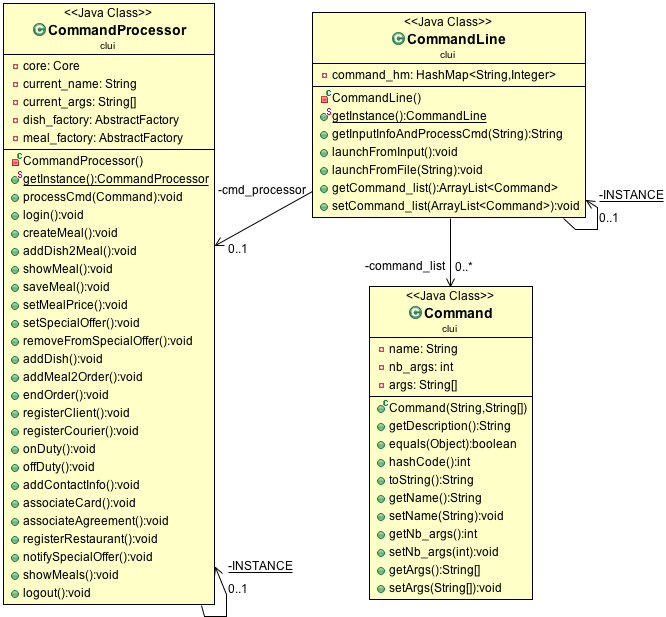
\includegraphics[scale=0.57]{./img/CLUI.png}
    \end{center}
  \caption{\umld of the command line user interface.}
  \label{fig:clui_uml}
\end{figure}

% subsection command_line_interface (end)

